\documentclass[11pt,xcolor=pdftex,dvipsnames,table,t]{beamer}
%adding handout above here kills pause
\usefonttheme[onlymath]{serif}
%\usetheme{default}
\usetheme{Hannover}
%\usepackage{times}
%\usefonttheme{structurebold}

\usepackage[english]{babel}
%\usepackage[table]{xcolor}
\usepackage{amsmath}
\usepackage{pgf,pgfarrows,pgfnodes,pgfautomata,pgfheaps}
\usepackage{amsmath,amssymb,setspace}
\usepackage[latin1]{inputenc}
\usepackage[T1]{fontenc}
\usepackage{relsize}
\usepackage{comment}

%RICH NOTE: this was causing errors for me
%\usepackage{pxfonts}

\usepackage[absolute,overlay]{textpos} 
\newenvironment{reference}[2]{% 
  \begin{textblock*}{\textwidth}(#1,#2) 
      \footnotesize\it\bgroup\color{red!50!black}}{\egroup\end{textblock*}} 

\DeclareMathSizes{10}{10}{6}{6} 

%rich added 
\setbeamertemplate{navigation symbols}{}
\setbeamertemplate{footline}[frame number]

\addtobeamertemplate{frametitle}{\vspace*{-.20cm}}{\vspace*{0.1cm}}

\usepackage{hyperref}
% Change the setup later on, after loading hyperref
\hypersetup{colorlinks=true, urlcolor=blue, linkcolor=blue, citecolor=blue, linktocpage}

% Bib stuff

\usepackage{natbib}
\usepackage{bibentry}
%\renewcommand{\cite}{\citet}
%\let\oldcite=\cite                                                          %\renewcommand{\cite}[1]{\textcolor[rgb]{0,0,1}{\oldcite{#1}}}
%\renewcommand{\cite}{\citet}



\title{Binary Choice}
\author{Richard L. Sweeney}
\institute{based on slides by Chris Conlon}
\date{Empirical Methods \\ Spring 2019}

\setbeamerfont{equation}{size=\tiny}
\DeclareMathSizes{10}{10}{6}{6} 

\begin{document}

\begin{frame}
    \titlepage
\end{frame}

\begin{frame}
    \tableofcontents  
\end{frame}

\section{Intro}

\begin{frame}
\frametitle{Binary Choice: Overview}
Many problems we are interested in look at discrete rather than continuous outcomes.
\begin{itemize}
       \item To move or not. 
       \item Entering a market.
       \item Getting married. 
       \item Going to college.
\end{itemize}
In this lecture we will 

\begin{itemize}
\item Review the well known limitations of the linear probability model (LPM)
\item Discuss interpretation of estimates of popular alternatives. 
\item Discussion options for dealing with endogeneity
\end{itemize}
\end{frame}

\section{LPM}

\begin{frame}{Linear Probability Model}
       OLS is called the \alert{linear probability model} 
       \begin{eqnarray*}
       Y_i  = \beta_0 + \beta_1 X_i + \varepsilon_i 
       \end{eqnarray*}
       because:
       \begin{eqnarray*}
       E[Y | X] &=& 1 \times Pr(Y=1 | X) + 0 \times Pr(Y=0  | X) \\
       Pr(Y=1 | X) &=& \beta_0 + \beta_1 X_i + \varepsilon_i
       \end{eqnarray*}
       The predicted value is a \alert{probability} and 
       \begin{eqnarray*}
       \beta_1 = \frac{Pr(Y=1 | X =x+\Delta x) - Pr(Y=1 | X=x)}{\Delta x}
       \end{eqnarray*}
       So $\beta_1$ represents the average change in probability that $Y=1$ for a unit change in $X$.
\end{frame}

\begin{frame}
       \frametitle{Well known problems}
       \begin{itemize}
       \item Constant marginals 
       \item Not bounded between 0 and 1
       \item Relatedly, literally cannot satisfy OLS condition that $\epsilon$ uncorrelated with $X$ for covariates with wide support. 
       \item Nevertheless .... 
       \end{itemize}
\end{frame}

\begin{frame}{Some well known textbooks}
(Baby) Wooldrige:
\begin{quote}
``Even with these problems, the linear probability model is useful and often applied in economics. It usually works well for values of the independent variables that are near the averages in the sample.'' (2009, p. 249)
\end{quote}
\begin{itemize}
\item Mentions heteroskedasticity of error (which is binomial given $X$) but does not address the violation of the first LSA.
\end{itemize}
\end{frame}

\begin{frame}{Some well known textbooks}
Angrist and Pischke (MHE) 
\begin{itemize}
\item several examples where marginal effects of probit and LPM are ``indistinguishable''.
\end{itemize}

\begin{quote}
...while a nonlinear model may fit the CEF (conditional expectation function) for LDVs (limited dependent variable models) more closely than a linear model, when it comes to marginal effects, this probably matters little. This optimistic conclusion is not a theorem, but as in the empirical example here, it seems to be fairly robustly true.(2009, p. 107)
\end{quote}
and continue...
\begin{quote}
...extra complexity comes into the inference step as well, since we need standard errors for marginal effects. (ibid.)
\end{quote}
\end{frame}

\begin{frame}
\frametitle{Counter example: Lewbel Dong and Yang (2012)}
\begin{itemize}
\item LPM is not just about taste and convenience.
\item Three treated observations, three untreated % \texttt{Treated=1}
\item Assume that $f(\varepsilon) \sim N(0,\sigma^2)$
\begin{eqnarray*}
D = I ( 1 + Treated + R + \varepsilon \geq 0 ) 
\end{eqnarray*}
\item Each individual treatment effect given by:
\begin{eqnarray*}
 I ( 2 + R + \varepsilon \geq 0 ) -  I ( 1 + R + \varepsilon \geq 0 )  =  I ( 0 \leq 1 + R + \varepsilon \leq 1 ) 
\end{eqnarray*}
\item All treatment effects are positive for all $(R,\varepsilon)$.
\item Construct a sample where true effect $=1$ for 5th individual, 0 otherwise. $ATE= \frac{1}{6}$.
\end{itemize}
\end{frame}

\begin{frame}[fragile]
\frametitle{Lewbel Dong and Yang (2012)}
\vspace{-10pt}
\tiny
\begin{semiverbatim}
. list
|     R   Treated   D |
1. |  -1.8         0   0 | 
2. |   -.9         0   1 |
3. |  -.92         0   1 |
4. |  -2.1         1   0 |
5. | -1.92         1   1 |
6. |    10         1   1 |

. reg D Treated R, robust

Linear regression                               Number of obs     =          6
                                          F(2, 3)           =       1.02
                                          Prob > F          =     0.4604
                                          R-squared         =     0.1704
                                          Root MSE          =     .60723

------------------------------------------------------------------------------
       |               Robust
       D |      Coef.   Std. Err.      t    P>|t|     [95% Conf. Interval]
-------------+----------------------------------------------------------------
Treated |  -.1550841   .5844637    -0.27   0.808    -2.015108     1.70494
       R |   .0484638   .0419179     1.16   0.331    -.0849376    .1818651
_cons |   .7251463   .3676811     1.97   0.143    -.4449791    1.895272
------------------------------------------------------------------------------
. nlcom _b[Treated]/_b[R]
_nl_1:  _b[Treated]/_b[R]
------------------------------------------------------------------------------
       D |      Coef.   Std. Err.      z    P>|z|     [95% Conf. Interval]
-------------+----------------------------------------------------------------
_nl_1 |       -3.2   10.23042    -0.31   0.754    -23.25125    16.85125
------------------------------------------------------------------------------
\end{semiverbatim}
\end{frame}

\begin{frame}[fragile]
\frametitle{Lewbel Dong and Yang (2012)}
\begin{itemize}
\item That went well, except that:
\begin{itemize}
\item we got the wrong sign of $\beta_T$
\item $\beta_1/\beta_2$ was the wrong sign and three times too big.
\end{itemize}
\item this is not because of small sample size or $\beta_1 \approx 0$.
\item As $n \rightarrow \infty$ we can get an arbitrarily precise wrong answer.
\item We don't even get the sign right!
\item This is still in OLS (not much hope for 2SLS).
\end{itemize}
\tiny
\begin{semiverbatim}
. expand 30
(...)
. reg D Treated R, robust

Linear regression                               Number of obs     =        180
                                          F(2, 177)         =      59.93
                                          Prob > F          =     0.0000
                                          R-squared         =     0.1704
                                          Root MSE          =       .433

------------------------------------------------------------------------------
       |               Robust
       D |      Coef.   Std. Err.      t    P>|t|     [95% Conf. Interval]
-------------+----------------------------------------------------------------
Treated |  -.1550841   .0760907    -2.04   0.043    -.3052458   -.0049224
       R |   .0484638   .0054572     8.88   0.000     .0376941    .0592334
_cons |   .7251463    .047868    15.15   0.000     .6306808    .8196117
\end{semiverbatim}
\end{frame}

\section{Logit/Probit}


\begin{frame}{Moving Away from LPM}
Problem with the LPM/OLS is that it requires that \alert{marginal effects are constant} or that probability can be written as linear function of parameters.
\begin{eqnarray*}
Pr(Y=1 | X) = \beta_0 + \beta_1 X+ \epsilon
\end{eqnarray*}

Want a function $F(z): (-\infty,\infty) \rightarrow [0,1]$.

What function will work?

\end{frame}

\begin{frame}{Choosing a transformation}
       \begin{itemize}
       \item One $F(\cdot)$ that works is $\Phi(z)$ the normal CDF. This is the \alert{probit} model.
       \begin{itemize}
       \item Actually any CDF would work but the normal is convenient.
       \end{itemize}
       \item Another $F(\cdot)$ that works is $\frac{e^z}{1+ e^z}=\frac{1}{1+e^{-z}}$ the logistic function . This is the \alert{logit} model.
       \item Both of these give `S'-shaped curves.
       \item This $F(\cdot)$ is often called a \alert{link function}. 
       \end{itemize}
\end{frame}


\begin{frame}
       \frametitle{A quick comparison}
       \begin{itemize}
       \item LPM prediction departs greatly from CDF long before $[0,1]$ limits.
       \item We get probabilities that are too extreme even for $X\hat{\beta}$ ``in bounds''.
       \item Logit and Probit are highly similar
       \end{itemize}
       \begin{center}
       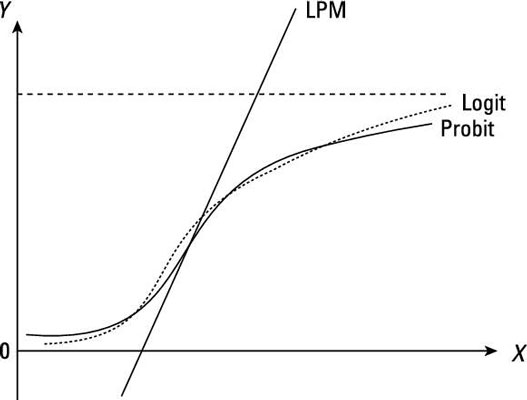
\includegraphics[width=2.5in]{resources/lpm-probit.jpg}
       \end{center}
\end{frame}

\begin{frame}
       \frametitle{We really care about marginal effects}
       \begin{center}
       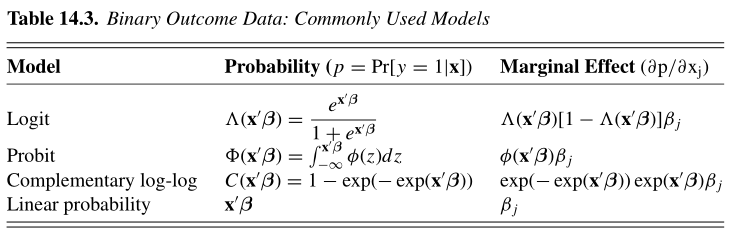
\includegraphics[width=\textwidth]{resources/CTmarginals}
       \end{center}
\end{frame}

\begin{comment}
\begin{frame}
       \frametitle{Latent Variables/ Limited Dependent Variables}
       An alternative way to think about this problem is that there is a continuously distributed $Y^{*}$ that we as the econometrician don't observe.
       \begin{eqnarray*}
       Y_i =
       \begin{cases}
       1 \mbox{ if } Y^{*} >0 \\
       0 \mbox{ if } Y^{*} \leq 0
       \end{cases}
       \end{eqnarray*}
       \begin{itemize}
       \item Instead we only see whether $Y^{*}$ exceeds some threshold (in this case $0$).
       \item We can think about $Y^{*}$ as a \alert{latent variable}.
       \item Sometimes you will see this description in the literature, everything else is the same!
       \end{itemize}
\end{frame}
       
       
\begin{frame}
       \frametitle{Index Models}
       We sometimes call these single index models or threshold crossing models
       \begin{eqnarray*}
       Z_i = X_i \beta
       \end{eqnarray*}
       \begin{itemize}
       \item We start with a potentially large number of regressors in $X_i$ but $X_i \beta = Z_i$ is a \alert{scalar}
       \item We can just calculate $F(Z_i)$ for Logit or Probit (or some other CDF).
       \item $Z_i$ is the \alert{index}. if $Z_i = X_i \beta$ we say it is a \alert{linear index} model.
       \end{itemize}
\end{frame}
\end{comment}

\begin{frame}
       \frametitle{Challenge: Where to evaluate?}
       \begin{eqnarray*}
       \frac{\partial E[Y_i | X_i] }{\partial X_{ik}} = f (X_i'\beta) \beta_k
       \end{eqnarray*}
       \begin{itemize}
       \item The whole point was that we wanted marginal effects not to be constant
       \item So where do we evaluate?
       \begin{itemize}
       \item Software often plugs in mean or median values for each component
       \item Alternatively we can integrate over $X$ and compute:
       $$
       E_{X_i}[ f (X_i'\beta) \beta_k]
       $$
       \item The right thing to do is probably to plot the response surface (either probability) or change in probability over all $X$.
       \end{itemize}
       \end{itemize}
\end{frame}

\begin{frame}
       \frametitle{How to compare across models?}

       Natural to compare log-Likelihood

       $$ L_N(\hat \beta) = \sum_i \left\{ y_i \ln \hat p_i + (1- y_i) \ln (1 - \hat p_i) \right\} $$

       \pause 
       What about the different marginals?
       
       \medskip
       Coefficients will be different because of the different formulas and normalizations. 
       
       \medskip
       According to CT, this works well for $0.1 < p < 0.9$

       \begin{eqnarray*}
              \hat \beta_{Logit} &\approx& 4 \hat \beta_{OLS} \\
              \hat \beta_{Probit} &\approx& 2.5 \hat \beta_{OLS} \\
              \hat \beta_{Logit} &\approx& 1.6 \hat \beta_{Probit}
       \end{eqnarray*}
\end{frame}

\begin{frame}
       \frametitle{A word of caution re interaction effects}
       \begin{itemize}
       \item Often we want to include interaction effects in our models. 
       $$ Y = \beta_1 x_1 + \beta_2 x_2 + \beta_{12}x_1x_2 + \epsilon $$ 
       \item A leading example is difference in differences 
       \item With LPM, interaction terms directly interpretable as the change in probabilities. 
       \item Conversely, \citet{ai2003interaction} show that the marginal of the interaction term has NO INTERPRETATION!
       \end{itemize}
\end{frame}


\begin{frame}
       \frametitle{Consider the probit}

       $$E[y|X] = \Phi(\beta_1 x_1 + \beta_2 x_2 + \beta_{12}x_1x_2) $$ 

       where $\Phi$ is the standard normal cdf. 

       \medskip

       Consider continuous $x_1$, $x_2$. The true interaction effect is 

       $$ \frac{\partial E[y|X]}{\partial x_1 \partial x_2} = 
              \beta_{12}\Phi'(\cdot) + (\beta_1 + \beta_{12}x_1)\Phi''(\cdot) $$ 

       \pause 
       However, most applied economists instead report the marginal effect of the interaction term, 
       $$\partial \Phi (\cdot)/ \partial (x_1 x_2) = \beta_{12} \Phi'(\cdot) $$

       Note that this can easily give the wrong sign, and that the true partial can be nonzero even if $\beta_{12} = 0$. 

\end{frame}

\section{Endogeneity}

\begin{frame}
\frametitle{What About Endogeneity?}

\cite{lewbel2012comparing} discuss four ``convenient'' options for binary choice models with endogenous regressors.
\begin{enumerate}
\item Close eyes, run the LPM with instruments (Suggested by MHE).
\item Specify the distribution of errors in first and second stage and do MLE (\texttt{biprobit} in STATA).
\item Control Function Estimation
\item `Special Regressor' Methods
\end{enumerate}
\end{frame}

\begin{frame}
\frametitle{Setup: Endogeneity}
Setup:
\begin{itemize}
\item Binary variable $D$: the outcome of interest
\item $X$ is a vector of observed regressors with coefficient $\beta$ 
\begin{itemize}
\item (Can think about $X^e$: endogenous and $X^0$: exogenous).
\item In a treatment model we might have that $T$ is a binary treatment indicator within $X$
\end{itemize}
\item $\epsilon$ is unobserved error. Specifying $f(e)$ can give logit/probit.
\item Threshold Crossing / Latent Variable Model:
\begin{eqnarray*}
D = \mathbf{1}(X \beta + \epsilon \geq 0)
\end{eqnarray*}
\item Goal is not usually $\hat{\beta}$ or it's CI, but rather $P(D=1 | X)$ or $\frac{\partial P[D=1 | x] }{\partial X}$ (marginal effects).
\end{itemize}
\end{frame}

\begin{frame}
\frametitle{Solution \#0 : LPM}
\vspace{-10pt}
\begin{block}{Advantages}
\vspace{-5pt}       
\begin{itemize}
\item Just like 2SLS.
\item Computationally easy (no numerical searches)
\item Missing $Z$ is about efficiency not consistency.
\item $X^e$ can be discrete or continuous (same estimator)
\item allows general heteroskedasticity (random coefficients)
\end{itemize}
\end{block}
\vspace{-5pt}       

\begin{block}{Disadvantages}
\vspace{-5pt}
\begin{itemize}
\item $\hat{F}_D$ is linear not S-shaped; can be outside $[0,1]$.
\item no element of $X$ can have $\infty$ support (e.g. no normally distributed regressors).
\item $\varepsilon$ not independent of any regressors  (even the exogenous ones). How do we also get $E[X^0 \varepsilon] =0$ ?
%\item Does not nest probit, logit, etc.. Can't compare efficiency
\end{itemize}
\end{block}
\end{frame}


\subsection{MLE}

\begin{frame}
\frametitle{Solution \#1 : MLE}
\begin{eqnarray*}
D = I ( X' \beta + \varepsilon \geq 0 ) \quad \mbox{and} \quad X^e = G(Z,\theta,e)
\end{eqnarray*}
\begin{itemize}
\item Fully specified $G$ (could be vector). Could be linear if $X^e$ continuous or probit if $X^e$ binary.
\item Need to fully specify distribution of $(\varepsilon,e, | Z)$, parametrized.
\item Implementation (see CT book), \texttt{biprobit} for joint normal in Stata.
\end{itemize}
\end{frame}


\begin{frame}
\frametitle{Solution \#1 : MLE}
\vspace{-10pt}
\begin{block}{Advantages}
\begin{itemize}
\item Nests logit, probit, etc. as special cases.
\item Can have any kind of $X^e$
\item Allows heteroskedasticity, random coefficients
\item Asymptotically efficient (if correctly specified)
\end{itemize}
\end{block}

\begin{block}{Disadvantages}
\begin{itemize}
\item Need to parametrize everything $G$, $F_{\varepsilon,e|Z}$.
\item Numerical optimization issues
\item Many nusiance parameters, sometimes poorly identified, especially with discrete $X^e$, correlation between latent $(\varepsilon,e)$.
\item Need to know all required instruments $Z$. Omitting just one $Z$ causes inconsistency in $G$. %(Not sure if something is exogenous, too bad!).
\end{itemize}
\end{block}
\end{frame}

\subsection{Control Functions}

       
\begin{frame}
\frametitle{Solution \#2 : Control Functions}
Setup: 
\begin{eqnarray*}
D &=& I ( X' \beta + \varepsilon \geq 0 ) 
\end{eqnarray*}
Assume first stage relationship identified and invertible in $e$
\begin{eqnarray*}
X^e &=& G(Z) +e  \quad \mbox{or}  \quad  X^e = G(Z,e)
\end{eqnarray*}
With conditions $ U \bot Z,e$
\begin{eqnarray*}
\varepsilon  &=&\lambda' e + U \quad \mbox{or}  \quad  \varepsilon = H(U,e) 
\end{eqnarray*}
       
Simple Case:
\begin{itemize}
\item Estimate a vector of functions $G$ in the $X^e$ models, get estimated errors $\hat{e}$.
\item Estimate the $D$ model including $\hat{e}$ as additional regressors in addition to $X$.
\item This ``cleans'' the errors in $U$.
\end{itemize}
\end{frame}

\begin{frame}[allowframebreaks]
       \frametitle{CF Example: Linear}
       From Wooldridge. Second stage: 
       $$y_1 = z_1'\delta + \alpha_1 y_2 + u_1$$ 

       $y_2$ is endogenous, but $E(z'u_1)=0$ 

       \medskip
       $z$ is L by 1 vector of instruments, with $z_1$ a strict subvector

       \medskip
       Write reduced form first stage as $$y_2 = z'\pi_2 + v_2$$ with $E(z'v_2)=0$

       \medskip
       Engogeneity of $y_2$ arises iff $u_1$ and $v_2$ are correlated.  

       \framebreak

       Write the projection $u_1 = \rho_1 v_2 + e_1$ 

       \medskip

       By definition, $E(v_2 e_1)=0$ and by construction $E(z'e_1)=0$ (because $z$ uncorrelated with $u$ and $v$). 

       \medskip

       We now have $$y_1 = z_1'\delta + \alpha_1 y_2 + \rho_1 v_2 + e_1$$

       Procedure
       \begin{enumerate}
              \item Regress $y_2$ on $z$ to recover $\hat v_2$ 
              \item Regress $y_1$ on $z_1, y_2, \mbox{and } \hat v_2$
       \end{enumerate}
       This regression is a \alert{control function} estimate. 
\end{frame}

\begin{frame}
\frametitle{Binary CF (Stata Version)}
\begin{itemize}
\item \texttt{ivprobit} assumes that $G(Z,e)$ is linear, and $(e,\varepsilon)$ jointly normal, independent of $Z$.
%\item not exactly the semi-parametric flexibility we were looking for...
\item It is actually Control Function not IV
\end{itemize}
\begin{eqnarray*}
D &=& I ( X^e  \beta_e + X^0 \beta_0+ \varepsilon \geq 0 ) \\
 X^e &=& \gamma Z + e  
\end{eqnarray*}
Run first-stage OLS and get residuals $\hat{e}$. Then plug into
\begin{eqnarray*}
D &=& I ( X^e  \beta_e + X^0 \beta_0 + \lambda \hat{e} + U  \geq 0 )
\end{eqnarray*}
and do a conventional probit estimator.
\begin{itemize}
%\item If you forget a $Z_2$ the resulting model isn't even probit!
\item God help you if $X^e$ isnt continuous.
\end{itemize}

\end{frame}

\begin{frame}
\frametitle{Stronger requirements than 2SLS}
\vspace{-10pt}
\begin{eqnarray*}
D &=& I ( X' \beta + \varepsilon \geq 0 ) ; \quad  X^e = G(Z,e) ,  \\
\varepsilon &=& H(U,e) \quad ; \quad U \bot X,e
\end{eqnarray*}
Much stronger requirements that 2SLS
\begin{itemize}
\item Must be able to solve for errors $e$ in $X^e$ equations (not just orthogonality)
\item Endogeneity must be caused only by $\varepsilon$ relation to $e$ so after conditioning on $e$ must be that $f(\varepsilon | e, X^{e}) = f( \varepsilon | e)$.
\item I need a consistent estimator for $e$ which means nothing is omitted.
\end{itemize}
Not Quite MLE
\begin{itemize}
\item First stage can be semi/non-parametric .
\item Don't need to fully specify joint distribution of $(\varepsilon,e)$ (Stata does though!).
\end{itemize}


\end{frame}


\begin{frame}
\frametitle{Control Functions: Advantages}
\begin{itemize}
\item Nests logit, probit, etc. as special cases
\item Requires less parametric information than MLE
\item Some versions are computationally easy without numerical optimization (Bootstrap!)
\item Less efficient than MLE due to less restrictions, but can be semiparametrically efficient given information.
\end{itemize}
\end{frame}

\begin{frame}
\frametitle{Control Functions (Disadvantages: Not well known)}
\begin{itemize}
%\item Only allows limited heteroskedasticity
\item Need to correctly specify vector $G(Z,e)$ including all $Z$. Omitting a $Z$ or misspecified $G$ causes inconsistency because we need to have joint conditions on $(\varepsilon , e)$.
\item Generally inconsistent for $X^e$ that is discrete, censored, limited, or not continuous.
\item If you cannot solve for a latent $e$ in $G(Z,e)$ then you can't get $\hat{e}$ for the censored observations (e.g.: $X^e = \max(0, Z'\gamma + e)$.
\item An observable $e$ is $e = X^e - E[X^e | Z]$ but for discontinuous $X^e$ that $e$ violates assumptions (except in very strange cases)
\begin{itemize}
\item Ex: $\varepsilon =  [ X^e - E[X^e | Z]] \lambda + U$ satisfies CF, but if $X^e$ is discrete then $e$ has some strange distribution that depends on regressors. 
\item Hard to generate a model of behavior that justifies this!
\end{itemize}
\end{itemize}
\end{frame}



\begin{frame}
\frametitle{Solution \#2 : Control Functions Generalized Residuals}
What if $X^e$ isn't continuous? Technically possible...
\begin{itemize}
\item Given the probit estimate in first stage we could construct a generalized residual (see Imbens and Wooldridge notes) 
\item $e^g \propto E[\varepsilon | Z, e]$. An estimate $\hat{e}^g$ of $e^g$ can be included as a regressor in the model to fix the endogeneity problem, just as $\hat{e}$ would have been used if the endogenous regressor were continuous.
\end{itemize}
Why would you ever want to do this..
\begin{itemize}
\item In the linear model we should just do IV with far fewer restrictions
\item In the nonlinear model, $\hat{e}^g$ requires almost as many assumptions as MLE which is efficient!
\end{itemize}
\end{frame}

\subsection{Special Regressors}
\begin{frame}
\frametitle{Solution \#3 : Special Regressor}
This section draws on \cite{dong2015simple}, 
\pause

but there are many other papers on this.... 

\small
Binary, ordered, and multinomial choice, censored regression, selection, and treatment models (Lewbel 1998, 2000, 2007a), truncated regression models (Khan and Lewbel 2007), binary panel models with FE (Honore and Lewbel 2002), dynamic choice models (Heckman and Navarro 2007, Abbring and Heckman 2007), contingent valuation models (Lewbel, Linton, and McFadden 2008), market equilibrium models of multinomial choice (Berry and Haile 2009a, 2009b), models with (partly) nonseparable errors (Lewbel 2007b, Matzkin 2007, Briesch, Chintagunta, and Matzkin 2009).\\
Other empirical applications: Anton, Fernandez Sainz, and Rodriguez-Poo (2002), Cogneau and Maurin (2002), Goux and Maurin (2005), Stewart (2005), Lewbel and Schennach (2007), and Tiwari, Mohnen, Palm, and van der Loeff (2007).\\
Precursors: Matzkin (1992, 1994) and Lewbel (1997).\\
Recent theory: Magnac and Maurin (2007, 2008) Khan and Tamer (2010), and Khan and Nekipelov (2010a, 2010b).
\end{frame}


\begin{frame}
\frametitle{Special Regressor: Requirements}
\begin{eqnarray*}
D &=& I ( X' \beta + V + \varepsilon \geq 0 )
\end{eqnarray*}
\vspace{-8pt}
\begin{itemize}
\item Exogenous $E[\varepsilon | V ] =0$ (Strict Exogeneity) \alert{This is the key!} 
\item Additively separable in the model
\begin{itemize}
       \item NOT interacted with other regressors.
       \item enters LINEARLY, e.g. $V$ must be continuously distributed after conditioning on other regressors 
\end{itemize}
\item Continuous distribution and large support (such as Normal)

\item Helpful to have thick-tails (kurtosis). Why? We want to trace $Pr(D | V)$ from $[0,1]$.
\item Can normalize its coefficient to $1$
\item 2SLS Assumptions: $E[ \varepsilon | Z] = 0$ and $E[Z'X]$ is full rank.
\end{itemize}
\end{frame}


\begin{comment}
\begin{frame}
\frametitle{Solution \#3 : Special Regressor: How it works}
\begin{enumerate}
\item Demean or center $V$ at zero. 
\item Assume that $f_v ( V | Z,X^e) = f_v(V | Z)$ and let $\hat{f}_v ( V | Z) $ be a nonparametric kernel estimator of $f_v(V | Z)$. Or just use a kernel of the whole thing $\hat{f}_v ( V | Z,X^e)$
\item For each observation $i$, Construct $\hat{T}_i = I [D_i -  I(V_i \geq 0)]/ \hat{f_v} (V_i | Z_i)$
\item Linear 2SLS regression of $\hat{T}$ on $X$ using instruments $Z$ to get the estimated coefficients $\hat{\beta}$.
\end{enumerate}
Here $\hat{f}_v(V|Z)$ is high dimensional. So will consider some simpler parametric or semi-parametric version of $f_v$.\\
By properly adjusting $T_i$ we guarantee to stay in $[0,1]$.
\end{frame}
\end{comment}

% from Dong, Lewbell and Yang
\begin{frame}
       \frametitle{A simple SR estimator}
       \begin{enumerate}
       \item Demean or center $V$ at zero. 
       \begin{itemize}
              \item Project $V$ onto all the instruments $Z$ and regressors $X$ to recover $\hat U_i = V_i - S_i'\hat b$  
       \end{itemize}
       \item Sort $n$ observations by $\hat U_i$. Then define $\hat f_i = 2/ \left[(\hat U_i^+ - \hat U_i^-) n \right]$ 
       \begin{itemize}
              \item this estimates the density using only the observations on either side of $i$
              \item alternatively, can use a kernel density estimator
       \end{itemize}
       \item Construct $\hat{T}_i = [D_i -  I(V_i \geq 0)]/ \hat{f_i}$
       \item Linear 2SLS regression of $\hat{T}$ on $X$ using instruments $Z$ to get the estimated coefficients $\hat{\beta}$.
       \end{enumerate}
       By properly adjusting $T_i$ we guarantee to stay in $[0,1]$.
\end{frame}
       
\begin{frame}
       \frametitle{Why does this work?}
       \begin{itemize}
       \item $V = S'b + U$ 
       \item Define $T = [ D - I(V \ge 0 ]/f(U) ] $
       \item Under these assumptions, can be shown that $T = X'\beta + \tilde \epsilon $ with $E(Z \tilde \epsilon) = 0$
       \item Therefore $E(ZT) = E(ZX')\beta$ 
       \end{itemize}
\end{frame}

\begin{frame}
\frametitle{Special Regressor Advantages}
\begin{itemize}
\item Unlike LPM it stays ``in bounds'' and is consistent with threshold crossing models.
\item Unlike MLE and CF, does not require correctly specified first stage model: any valid set of instruments may be used, with only efficiency at stake.
\item Unlike MLE, the SR method has a linear form, not requiring iterative search
\item Unlike CF, the SR method can be used when endogenous regressors $X^e$ are discrete or limited; unlike ML there is a single estimation method, regardless of the characteristics of $X^e$
\item Unlike MLE, the SR method permits unknown heteroskedasticity in the model errors.
\end{itemize}
\end{frame}

\begin{frame}
\frametitle{Special Regressor Disadvantages}
\begin{itemize}
\item Because assumptions are weaker we give up a lot of potential efficiency (larger SEs).
\item Of course this presumes the assumptions were valid and alternatives were consistent.
\item SR Methods are generally valid under more general conditions.
\end{itemize}
\end{frame}

\begin{frame}
\frametitle{ The average index function (AIF)/ Propensity Score}
In the original problem
\begin{eqnarray*}
D &=& I ( X' \beta + \varepsilon \geq 0 )
\end{eqnarray*}
\begin{itemize}
\item $V$ is part of $X$ with coefficient $=1$
\item When $\varepsilon \bot x$ write the propensity score: $E[D | X] = E[D | X \beta] = F_{-\varepsilon} (X \beta)  = Pr(- \varepsilon \leq X \beta)$. 
\item Under independence $X \bot \varepsilon$ these are the same, under endogeneity or even heteroskedasticity they are not.
\end{itemize}
\end{frame}

\begin{frame}
\frametitle{ The average index function (AIF)/ Propensity Score}
\begin{itemize}
\item Blundell and Powell (ReStud 2004, this is actually the most important control function paper) use the average structural function (ASF) $= F_{-\varepsilon} (X \beta) $ to summarize choice probabilities. But when $\varepsilon \bot X$ is violated then they have to compute $F_{-\varepsilon | X} (X \beta) $ which is quite difficult (especially semiparametrically).
\item Lewbel, Dong and Tang (CJE 2012) propose using the AIF estimator $E[D | X \beta]$ instead.
\item Like ASF the AIF is based on the estimated index $X \beta$ and is equal to the propensity score if $\varepsilon \bot X$. However, when this is violated (endogeneity, heteroskedasticity) the AIF is easier to estimate, via unidimensional nonparametric regression of $D$ on $X \beta$.
\end{itemize}
\end{frame}

\begin{frame}
\frametitle{ What is the difference}
\begin{description}
\item[Propensity Score: ]  Conditions on ALL covariates using $F_{-\varepsilon | X}$.
\item[ASF: ]  Conditions on no covariates using $F_{-\varepsilon }$.
\item[AIF: ]  Conditions on index only  using $F_{-\varepsilon | X \beta}$.
\end{description} 

\begin{itemize}
\item Unlike ASF, AIF is always identified and easy to estimate.
\item Unlike Propensity score AIF uses $\beta$ and isn't high dimensional
\item ASF, AIF and propensity score all coincide under exogeneity.
\end{itemize}
\end{frame}

\begin{frame}
\frametitle{ Marginal Effects}
\begin{itemize}
\item With exogenous $X$: MFX are $m(X) = p'(X) =  \frac{\partial E[D | X \beta]}{\partial X}$.
\item Let $f_{-\varepsilon}$ be marginal pdf of $-\varepsilon$. If $D=I(X' \beta + \varepsilon \geq 0)$ with $\varepsilon \bot X$ then:
\end{itemize}
\begin{eqnarray*}
m (X \beta) \beta= \frac{\partial E[D | X]}{\partial X}  = \frac{\partial E[D | X \beta]}{\partial X' \beta}  \beta  = f_{-\varepsilon}(X' \beta) \beta
\end{eqnarray*}

With endogenous $X$:
\begin{itemize}
\item Propensity Score marginal effects are $m(X) = p'(X) =  \frac{\partial E[D | X]}{\partial X}$.
\item ASF marginal effects are $m(X) =\frac{\partial ASF(X'\beta)}{\partial X'\beta} \beta = f_{-\varepsilon}(X' \beta) \beta.$
\item AIF marginal effects are $m(X) =\frac{\partial ASF(X'\beta)}{\partial X'\beta} \beta = \frac{\partial E[D | X' \beta ]}{\partial X' \beta} \beta$
\end{itemize}
Given $\hat{\beta}$ ASF and AIF mfx require just one dimensional index derivative.
\end{frame}

\begin{frame}
\frametitle{Binary Choice with Endogenous Regressors}
\begin{itemize}
\item Linear probability models, Maximum Likelihood, and Control functions (including \texttt{ivprobit} have more drawbacks and limitations than are usually recognized.
\item Special Regressor estimators are a viable alternative (or at least they have completely different drawbacks and may be more generally applicable than has been recognized).
\item In practice, best might be to try all estimators and check robustness of results. Can use marginal effects to normalize them the same when comparing.
\item Average Index Functions can be used to construct estimated probabilities and comparable marginal effects across estimators, often simpler to calculate than Average Structural Functions.
\item Implementation of special regressor in Stata is done in \texttt{sspecialreg}.
\end{itemize}
\end{frame}

\begin{frame}
\frametitle{Empirical Example: Dong and Lewbel (2015)}
\begin{itemize}
\item Binary dependent variable: does $i$ migrate from one state to another. 
\item Special Regressor $V_i$: age. Human capital theory suggests it should appear linearly (or at least monotonic) in a threshold crossing model 
\item Migration is drive by maximizing expected lifetime income and potential gain from a permanent change in income declines linearly in age.
\item $V_i$ is defined as negative of age, demeaned so that coefficient is positive with mean zero.
\item Other endogenous regressors: family income pre migration, home ownership.
\end{itemize}
\end{frame}

\begin{frame}
\frametitle{Empirical Example: Dong and Lewbel (2015)}
As a reminder, normally we would be in trouble here:
\begin{itemize}
\item MLE would be very complicated with multiple endogenous variables
\item Control functions \texttt{ivprobit} won't work with 0/1 homeowner variable.
\end{itemize}
\end{frame}

\begin{frame}
\frametitle{Empirical Example: Dong and Lewbel (2015)}
1990 PSID
\begin{itemize}
\item male head of household (23-59 years), completed education and not-retired (key!)
\item $D=1$ indicates migration during 1991-1993.
\item 4689 Individuals, 807 migrants.
\item Exogenous regressors: years of education, \# of children, white, disabled, married.
\item Instruments: level of govt benefits in 1989-1990, state median residential tax rate.
\end{itemize}
\end{frame}

\begin{frame}
\frametitle{Empirical Example: Dong and Lewbel (2015)}
Specifications
\begin{itemize}
\item Special Regressors: kernel density vs. sorted data density.
\item Special Regressor: homoskedastic vs. heteroskedastic errors.
\item LPM vs 2SLS
\item Probit (assuming exogeneity)
\item Control Function (\texttt{ivprobit}) misspecified for \texttt{homeowner} endogenous binary variable.
\end{itemize}
\end{frame}


\begin{frame}
\frametitle{Empirical Example}
\begin{center}
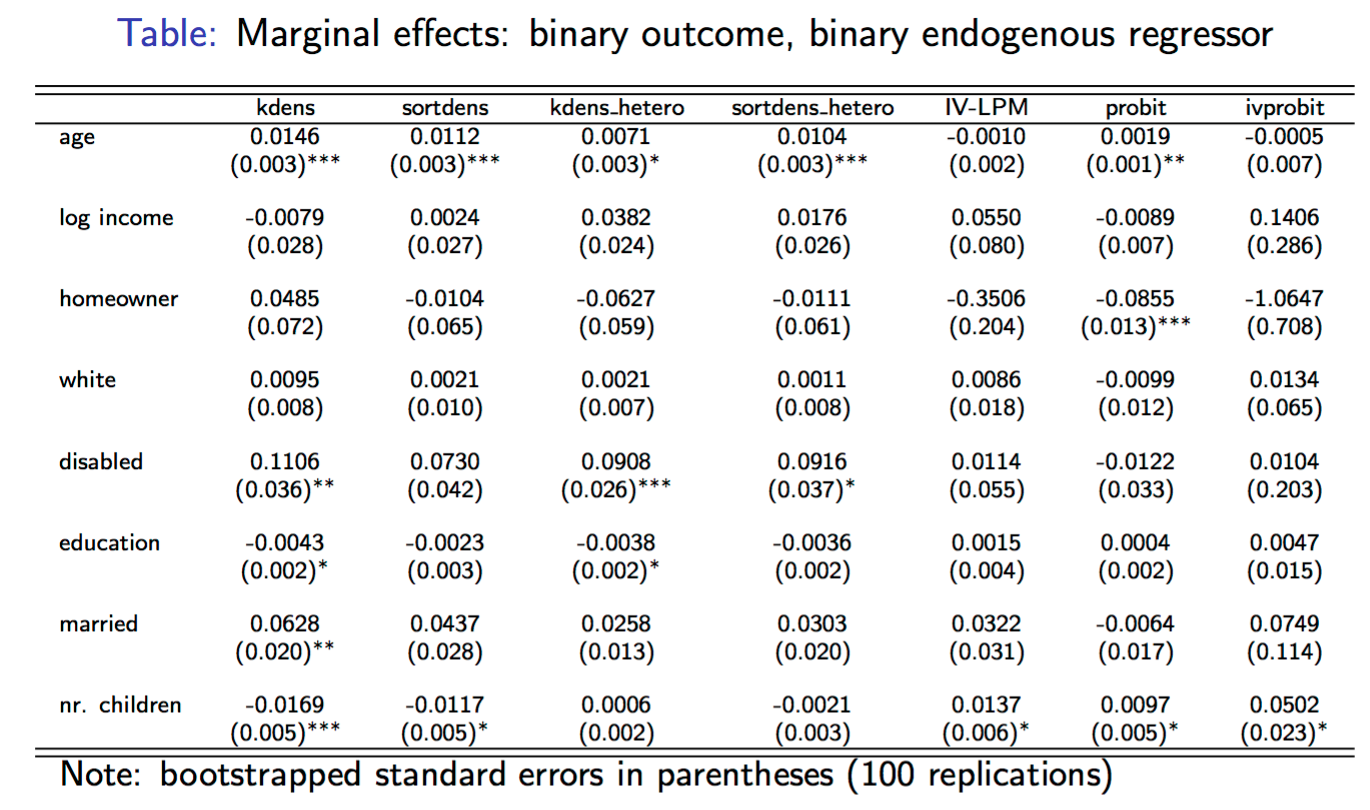
\includegraphics[width=4in]{resources/specialregtable.png}
\end{center}
\end{frame}

\begin{frame}
\frametitle{Empirical Example: Dong and Lewbel (2015)}

\begin{itemize}
\item SEs of MFX are computed from 100 bootstrap replications
\item MFX of special regressor (age) is estimated as positive and significant but LPM and ivprobit estimate negative effects!
\item household income and home ownership status do not seem to play significant roles in migration decision.
\item Kernel density estimator seems to give most significant results.
\end{itemize}
\end{frame}


%%%%%%%%%%%%%%%%%%%%%%%%%%%%%%%%%%%%%%%%%%%%%%%%%%%%%%%%%%%%%%%%%%%%%
\begin{frame}[allowframebreaks]
       \bibliographystyle{jpe}
       \bibliography{../empirical-methods}
\end{frame}

%%%%%%%%%%%%%%%%%%%%%%%%%%%%%%%%%%%%%%%%%%%%%%%%%%%%%%%%%%%%%%%%%%%%%%
\section*{Backup}
          
\end{document}
